\documentclass[a4paper]{article}

\usepackage[swedish]{babel}
\usepackage[utf8x]{inputenc}
\usepackage{amsmath}
\usepackage{amssymb}
\usepackage[T1]{fontenc}
\usepackage{graphicx}
\usepackage{epstopdf}
\usepackage{bm}
\usepackage{mathtools}
\usepackage{gauss}
\usepackage{placeins} %FloatBarrier

\newcommand{\mat}[1]{\bm{\mathit{#1}}}

\newcommand{\mline}{%
  \hspace{-\arraycolsep}%
  \strut\vrule
  \hspace{-\arraycolsep}%
}

\begin{document}

\section*{1.1}
\subsection*{a)}

Bestäm alla egenvärden och egenvektorer till matrisen

\begin{equation*}
  \mat{A} = 
  \begin{bmatrix}
    11 & -6 \\
    12 & -6
  \end{bmatrix}.
\end{equation*}

Egenvärdena för matrisen $\mat{A}$ fås enligt sats 3.3 som nollställena till den
karekteristiska ekvationen

\begin{align*}
  &p_{\mat{A}}(\lambda) = \det(\mat{A} - \lambda\mat{I}) = (11 - \lambda)(-6 - \lambda) + 6\cdot 12 = 0\\
  &\iff \lambda^2 - 5\lambda + 6 = 0 \iff \lambda_{1,2} = \frac{5}{2} \pm \frac{1}{2} = \begin{cases}
    3\\
    2
    \end{cases}.
\end{align*}

\noindent För $\lambda_1 = 3$ fås den första egenvektorn som lösningen till

\begin{align*}
  &(\mat{A} - \lambda_1\mat{I})\vec{s_1} = 0\\
  \vspace{1cm}\\
  &\Rightarrow \begin{gmatrix}[p]
    8 & -6 & \mline & 0\\
    12 & -9 & \mline & 0
    \rowops
    \add[-3/2]{0}{1}
    \end{gmatrix}
  &\Rightarrow \begin{gmatrix}[p]
    8 & -6 & \mline & 0\\
    0 & 1 & \mline & t
    \rowops
    \add[6]{1}{0}
  \end{gmatrix}
  &\Rightarrow \begin{gmatrix}[p]
    1 & 0 & \mline & \frac{6}{8}t\\
    0 & 1 & \mline & t
  \end{gmatrix}\\
  \vspace{1cm}\\
  & \Rightarrow \vec{s_1} = t\begin{bmatrix}
    6\\
    8
   \end{bmatrix}.
\end{align*}

\noindent På liknande sätt fås egenvektorn för $\lambda_2 = 2$ som

\begin{align*}
  &(\mat{A} - \lambda_2\mat{I})\vec{s_2} = 0\\
  \vspace{1cm}\\
  &\Rightarrow \begin{gmatrix}[p]
    9 & -6 & \mline & 0\\
    12 & -8 & \mline & 0
    \rowops
    \add[-4/3]{0}{1}
    \end{gmatrix}
  &\Rightarrow \begin{gmatrix}[p]
    9 & -6 & \mline & 0\\
    0 & 1 & \mline & t
    \rowops
    \add[6]{1}{0}
  \end{gmatrix}
  &\Rightarrow \begin{gmatrix}[p]
    1 & 0 & \mline & \frac{6}{9}t\\
    0 & 1 & \mline & t
  \end{gmatrix}\\
  \vspace{1cm}\\
  & \Rightarrow \vec{s_2} = t\begin{bmatrix}
    6\\
    9
   \end{bmatrix}.
\end{align*}

\subsection*{b)}

\begin{equation*}
  \begin{cases}
    x'_1(t) = 11x_1(t) - 6x_2(t)\\
    x'_2(t) = 12x_1(t) - 6x_2(t)
  \end{cases}
  \iff
  \vec{x'} = \mat{A}\vec{x},
\end{equation*}
där
\begin{equation*}
  \vec{x'} = \begin{bmatrix}
    x'_1\\
    x'_2
  \end{bmatrix}, \vec{x} = \begin{bmatrix}
    x_1\\
    x_2
    \end{bmatrix}.
\end{equation*}

\noindent Vektorerna $\vec{s_1}$ och $\vec{s_2}$ är linjärt oberoende, vilket
medför att matris $\mat{A}$ är diagonaliserbar enligt sats 3.6. Därefter ger
sats 3.8 den allmänna lösningen till systemet på formen

\begin{equation*}
  \vec{x} = c_1e^{3t}\begin{bmatrix}6\\8\end{bmatrix} + c_2e^{2t}\begin{bmatrix}6\\9\end{bmatrix}
  \iff \begin{cases}
    x_1(t) = 6c_1e^{3t} + 6c_2e^{2t}\\
    x_2(t) = 8c_1e^{3t} + 9c_2e^{2t}
    \end{cases}
\end{equation*}

\subsection*{c)}

För stora $t$ så är $e^{2t} \approx e^{3t}$, förhållandet mellan $x_1(t)$ och
$x_2(t)$ kan då skrivas som

\begin{equation*}
  \frac{x_1(t)}{x_2(t)} = \frac{6(c_1e^{3t} + c_2e^{2t})}{8c_1e^{3t} + 9c_2e^{2t}} \approx \frac{1}{\frac 86 + \frac 96},
\end{equation*}

\noindent där bråken i nämnaren kan återfinnas som förhållandet mellan
komponenterna i egenvektorerna.

\section*{1.2}

\subsection*{a)}

En \textsc{Matlab}-utskrift för egenvärdena till matrisen $\mat{B}$ som ges enligt
uppgiften kan ses nedan

\FloatBarrier
\begin{figure}[h!]
  \centering
  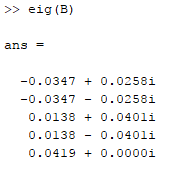
\includegraphics[width=0.35\linewidth]{figurer/matlab_1_2_a.png}
  %\caption{}
\end{figure}
\FloatBarrier

\noindent \text{Matlab} hittar 5 stycken egenvärden, och eftersom $\mat{B}$ är en
$5\times 5$ matris ger sats 3.9 att matrisen är diagonaliserbar.

Utförs samma räkning med \textsc{Maple} fås istället (egenvektorerna markeras
med blå text)

\FloatBarrier
\begin{figure}[h!]
  \centering
  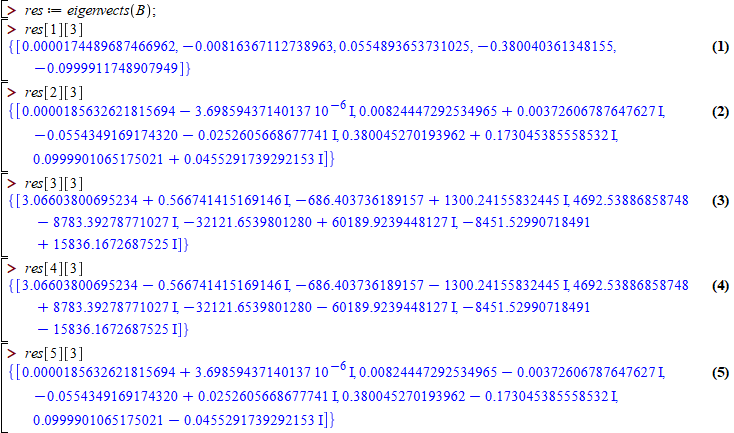
\includegraphics[width=\linewidth]{figurer/maple_1_2_a1.png}
  %\caption{}
\end{figure}
\FloatBarrier

\noindent Om egenvektorerna sedan samlas i en matris $\mat{S}$ så kan
determinanten beräknas för att avgöra om egenvektornerna som \textsc{Maple} ger
är linjärt oberoende.

\FloatBarrier
\begin{figure}[h!]
  \centering
  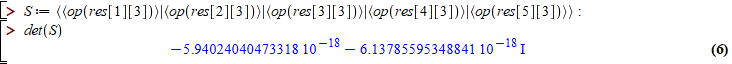
\includegraphics[width=\linewidth]{figurer/maple_1_2_a2.png}
  %\caption{}
\end{figure}
\FloatBarrier

\noindent Eftersom  determinanten är skild från noll är de 5 egenvektornerna linjärt
oberoende, vilket medför att matrisen $\mat{B}$ är diagonaliserbar enligt sats 3.6.

\subsection*{b)}

Egenvärdena som \textsc{Matlab} hittar till matrisen $\mat{A}$ som uppgiften ger
beräknas nedan

\FloatBarrier
\begin{figure}[h!]
  \centering
  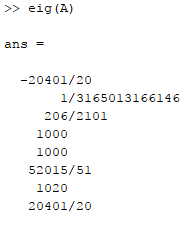
\includegraphics[width=0.35\linewidth]{figurer/matlab_1_2_b.png}
  %\caption{}
\end{figure}
\FloatBarrier

\noindent Eftersom \textsc{Matlab} ger 7 stycken olika egenvärden så är matrisen
inte diagonaliserbar enligt sats 3.9 (då matrisen $\mat{A}$ är $8\times 8$).

Sedan utförs samma räkning i \textsc{Maple} som istället ger att matrisen
$\mat{A}$ har 8 stycken linjärt oberoende egenvektorer (se nedanstående figur)
samt att determinanten hos egenvektorsmatrisen är nollskild. Detta ger istället
att matrisen $\mat{A}$ skulle vara diagonaliserbar enligt sats 3.6.

Anledningen till denna skillnad är att matrisen $\mat{A}$ är den så kallade
rosser-matrisen som är särskilt utformad för att testa algoritmer som beräknar
egenvärden och egenvektorer hos en matris. Enligt definitionen av
rosser-matrisen är 1000 ett dubbelt egenvärde, vilket medför att matrisen inte
är diagonaliserbar enligt sats 3.9.

\FloatBarrier
\begin{figure}[h!]
  \centering
  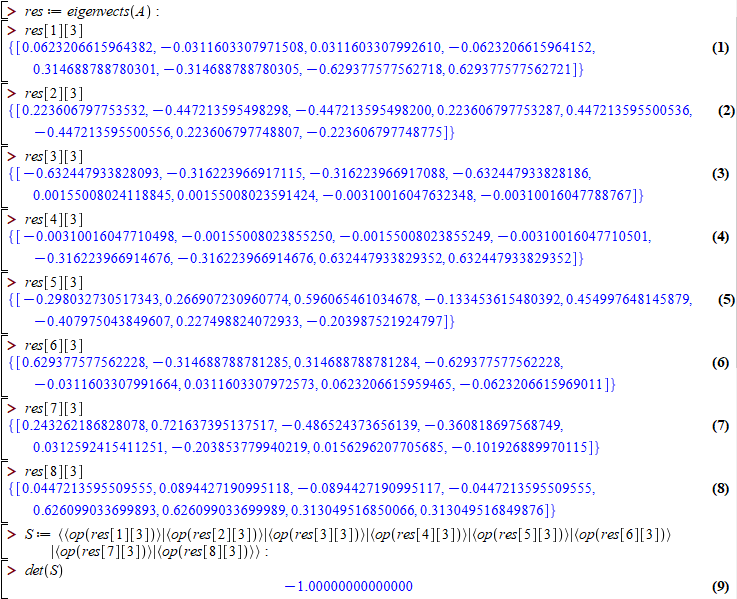
\includegraphics[width=\linewidth]{figurer/maple_1_2_b.png}
  %\caption{}
\end{figure}
\FloatBarrier

\section*{1.3}
\subsection*{a)}

Enligt uppgiften gäller

\begin{equation*}
  \frac{\text{d}\vec{x}}{\text{d}t} = \mat{A}\vec{x} + \vec{f}(t), \quad \mat{A} = \begin{bmatrix}-11 & 6\\-12 & 6\end{bmatrix}, \vec{f}(t) = \begin{bmatrix}3\\4\end{bmatrix}e^{-it},
\end{equation*}

\noindent Notera att systemmatrisen $\mat{A}$ är den negativa systemmatrisen
från uppgift 1.1 a), egenvektorerna fås därmed som

\begin{equation*}
  \lambda = \begin{cases}-3\\-2\end{cases}
\end{equation*}

\noindent Eftersom egenvektorerna skiljer sig från insignalens frekvens så ger
sats 4.6 den stataionära lösningen till systemet

\begin{align*}
  \vec{x_P}(t) &= ((-i)\mat{I} - \mat{A})^{-1}\begin{bmatrix}3\\4\end{bmatrix}e^{-it} = \begin{bmatrix}11-i & -6\\12 & -6-i\end{bmatrix}^{-1}\begin{bmatrix}3\\4\end{bmatrix}e^{-it}\\[2ex]
  &= \frac{1}{5-5i}\begin{bmatrix}-6-i & 6\\ -12& 11 - i\end{bmatrix}\begin{bmatrix}3\\4\end{bmatrix}e^{-it}\\[2ex]
  &= \frac{1}{5-5i}\begin{bmatrix}4-3i\\8-4i\end{bmatrix}e^{-it}
\end{align*}

\subsection*{b)}

Återigen eftersom $\mat{A}$ är den negativa systemmatrisen till systemet i
uppgift 1.1 a) så fås egenvärden samt egenvektorer som

\begin{equation*}
  \lambda = \begin{cases}-3\\-2\end{cases}, \mat{S} = -\begin{bmatrix}6 & 6\\8 & 9\end{bmatrix},
\end{equation*}
  
\noindent sats 3.8 ger då den homogena lösningen till systemet

\begin{equation*}
  \vec{x_H} = -c_1e^{-3t}\begin{bmatrix}6\\8\end{bmatrix} - c_2e^{-2t}\begin{bmatrix}6\\9\end{bmatrix}
\end{equation*}

\noindent Den totala lösningen ges då av

\begin{equation*}
  \vec{x} = \vec{x_H} + \vec{x_P} = \underbrace{-c_1e^{-3t}\begin{bmatrix}6\\8\end{bmatrix} - c_2e^{-2t}\begin{bmatrix}6\\9\end{bmatrix}}_{\text{Transient}} + \underbrace{\frac{1}{5-5i}\begin{bmatrix}4-3i\\8-4i\end{bmatrix}e^{-it}}_{\text{Stationär}}.
\end{equation*}

\section*{1.4}

Systemet för fågelpopulationen över tid ges som

\begin{equation*}
  \begin{cases}
    x_{n+1} = 0x_n + ky_n\\
    y_{n+1} = 0.8x_n + 0.6y_n
  \end{cases}, n = 0, 1, 2, \ldots
\end{equation*}

\noindent Rekursionsekvationerna för $x$ och $y$ beskriver i detta fall
derivatan av variablerna i diskreta tidsintervall på 1 år. Ur systemmatrisen

\begin{equation*}
  \mat{A} = \begin{bmatrix}0 & k \\ 0.8 & 0.6 \end{bmatrix}
\end{equation*}

\noindent fås egenvärdena som nollställena till det karekteristiska polynomet
(enligt sats 3.3)

\begin{align*}
  p_A(\lambda) &= (0-\lambda)(0.6 - \lambda) - 0.8k = 0 \iff \lambda^2 - 0.6\lambda - 0.8k = 0\\
               &\iff (\lambda - 0.3)^2 - 0.09 + 0.8k = 0\\
               &\iff \lambda = 0.3 \pm \sqrt{0.09 + 0.8k}.
\end{align*}

Begynnelsevilkoret i uppgiften ger här att koefficienterna $c_1$ och
$c_2$ i lösningen till systemet alltid är nollskilda.

\subsection*{a)}

$k = \frac 15$ ger egenvärdena $\lambda_1 = 0.8$ och $\lambda_2 = -0.2$. Eftersom
det största egenvärden är större än 0 så växer populationen obegränsat (enligt
sats 4.2). Lägg märke till att $\lambda_2 < 0$ vilket medför att termen
$c_ke^{\lambda_2t}\vec{s_2} \to 0, t\to \infty$

\begin{align*}
  (\mat{A} - \lambda_1\mat{I})\vec{s_1} = 0 &\Rightarrow
  \begin{gmatrix}[p]
    -0.8 & 0.2 & \mline & 0\\
    0.8 & -0.2 & \mline & 0
    \rowops
    \add[1]{0}{1}
  \end{gmatrix}
  \Rightarrow
  \begin{gmatrix}[p]
    -0.8 & 0.2 & \mline & 0\\
    0 & 1 & \mline & t
    \rowops
    \add[-0.2]{1}{0}
  \end{gmatrix}\\
  &\Rightarrow
  \begin{gmatrix}[p]
    1 & 0 & \mline & \frac 14 t\\
    0 & 1 & \mline & t
  \end{gmatrix}\\
  &\Rightarrow \vec{s_1} = t\begin{bmatrix}1\\4\end{bmatrix}
\end{align*}.

\noindent Sats 3.8 ger den slutliga lösningen, som för stora $t$ kan uppskattas
som 

\begin{align*}
  \begin{bmatrix}x\\y\end{bmatrix} \approx c_1e^{0.8t}\begin{bmatrix}1\\4\end{bmatrix} + 0
\end{align*}

\noindent För stora $t$ finns då approximativt $2$ gånger så många vuxna som kycklingar.

\subsection*{b)}

På samma sätt som i förra uppgiften ger $k = \frac 12$ egenvärdena $\lambda_1 =
1$ och $\lambda_2 = -0.4$. Återigen så växer populationen obegränsat (enl. sats
4.2) då $lambda_1 > 0$ Egenvektorerna fås som 

\begin{align*}
  (\mat{A} - \lambda_1\mat{I})\vec{s_1} = 0 &\Rightarrow
  \begin{gmatrix}[p]
    -1 & 0.5 & \mline & 0\\
    0.8 & -0.4 & \mline & 0
    \rowops
    \add[0.8]{0}{1}
  \end{gmatrix}
  \Rightarrow
  \begin{gmatrix}[p]
    -1 & 0.5 & \mline & 0\\
    0 & 1 & \mline & t
    \rowops
    \add[-0.5]{1}{0}
  \end{gmatrix}\\
  &\Rightarrow
  \begin{gmatrix}[p]
    -1 & 0 & \mline & -0.5t\\
    0 & 1 & \mline & t
  \end{gmatrix}\\
  &\Rightarrow \vec{s_1} = t\begin{bmatrix}1\\2\end{bmatrix}
\end{align*}.

\noindent Eftersom $\lambda_2 < 0$ så går termen $c_2e^{\lambda_2t}\vec{s_2} \to 0, t \to
\infty$ (m.h.a. stats 3.8). För stora $t$ ser lösningen ungefär ut som 

\begin{align*}
  \begin{bmatrix}x\\y\end{bmatrix} \approx c_1e^{t}\begin{bmatrix}1\\2\end{bmatrix} + 0
\end{align*}

\noindent För stora finns då 2 gånger så många vuxna som kycklingar.

\subsection{c)}

Här ger $k = 2$ egenvärdena $\lambda_1 = 1.6$ och $\lambda_2 = -1$. Eftersom
$\lambda_1 > 0$ så växer populationen obegränsat (sats 4.2). Egenvektorn för
$\lambda_1$ blir

\begin{align*}
  (\mat{A} - \lambda_1\mat{I})\vec{s_1} = 0 &\Rightarrow
  \begin{gmatrix}[p]
    -1.6 & 2 & \mline & 0\\
    0.8 & -1 & \mline & 0
    \rowops
    \add[0.5]{0}{1}
  \end{gmatrix}
  \Rightarrow
  \begin{gmatrix}[p]
    -1.6 & 2 & \mline & 0\\
    0 & 1 & \mline & t
    \rowops
    \add[-2]{1}{0}
  \end{gmatrix}\\
  &\Rightarrow
  \begin{gmatrix}[p]
    -1.6 & 0 & \mline & -2t\\
    0 & 1 & \mline & t
  \end{gmatrix}\\
  &\Rightarrow \vec{s_1} = t\begin{bmatrix}5\\4\end{bmatrix}
\end{align*}.

\noindent Då $\lambda_2 < 0$ så blir termen $c_2e^{\lambda_2t}\vec{s_2} \to 0, t \to
\infty$ försumbar i lösningen som ges av sats 3.8. För stora $t$ få ungefärligt

\begin{align*}
  \begin{bmatrix}x\\y\end{bmatrix} \approx c_1e^{1.6t}\begin{bmatrix}5\\4\end{bmatrix} + 0
\end{align*}

\noindent Det kommer då finnas $\frac 54 = 1.25$ kycklingar för varje vuxen.

\section*{1.5}

Enligt uppgiften skall $e^{\mat{A}t}$ beräknas för

\begin{equation*}
  \mat{A} = \begin{bmatrix} 11 & -6\\ 12 & -6\end{bmatrix}.
\end{equation*}

\noindent Uppgift 1.1 ger $\lambda_1 = 3, \lambda_2 = 2$ samt

\begin{equation*}
  \mat{S} = \begin{bmatrix}6 & 6\\8 & 9\end{bmatrix}, \Lambda = \begin{bmatrix}3 & 0\\0 & 2\end{bmatrix}.
\end{equation*}

\noindent Inversen till $\mat{S}$ fås som

\begin{equation*}
  \mat{S}^{-1} = \frac{1}{\det(\mat{S})}\text{adj}(\mat{S}) = \frac 16 \begin{bmatrix}9 & -6\\-8 & 6\end{bmatrix}.
\end{equation*}

\noindent Härefter kan Definition 5.2 användas för att beräkna $e^{\mat{A}t}$

\begin{align*}
  e^{\mat{A}t} &= \mat{S}e^{\Lambda t}\mat{S}^{-1} = \frac 16 \begin{bmatrix}6 & 6\\8 & 9\end{bmatrix}\begin{bmatrix}e^{3t} & 0\\0 & e^{2t}\end{bmatrix}\begin{bmatrix}9 & -6\\-8 & 6\end{bmatrix}\\[2ex]
               &= \frac 16 \begin{bmatrix}6 & 6\\8 & 9\end{bmatrix}\begin{bmatrix}9e^{3t} & -6e^{3t}\\-8e^{2t} & 6e^{2t}\end{bmatrix}\\[2ex]
               &= \frac 16 \begin{bmatrix}9\cdot 6e^{3t} - 8\cdot 6e^{2t} & -6\cdot 6e^{3t} + 6\cdot 6e^{2t}\\9\cdot 8e^{3t} - 9\cdot 8e^{2t} & -6\cdot 8e^{3t} + 9\cdot 6e^{2t}\end{bmatrix}\\[2ex]
               &= \begin{bmatrix}9e^{3t} - 8e^{2t} & 6\left( e^{2t} - e^{3t} \right)\\12\left( e^{3t} - e^{2t} \right) & 9e^{2t} - 8e^{3t}\end{bmatrix}.
\end{align*}

\subsection*{b)}

\section*{1.6}

\begin{equation*}
  \mat{A} = 2\pi\begin{bmatrix}0 & 4\\-1 & 0\end{bmatrix},\quad \mat{B} = 2\pi\begin{bmatrix}0 & 1\\-4 & 0\end{bmatrix}.
\end{equation*}

\subsection*{a)}

Det karekteristiska polynomet för $\mat{A}$ ger egenvärdena

\begin{align*}
  p_A(\lambda) &= (-\lambda)^2 + 4 = 0 \iff \lambda = \pm 2i
                 &\Rightarrow \mat{\Lambda} = 2\pi\begin{bmatrix}2i & 0\\0 & -2i\end{bmatrix}.
\end{align*}

\noindent Exponentialmatrisen för $\mat{\Lambda}$ blir då

\begin{equation*}
  e^{\mat{\Lambda}} = \begin{bmatrix}e^{i4\pi} & 0\\0 & e^{-i4\pi}\end{bmatrix} = \begin{bmatrix}1 & 0\\0 & 1\end{bmatrix}.
\end{equation*}

\subsection*{b)}

Exponentialmatrisen för $\mat{A}$ kan då beräknas m.h.a. Definition 5.2

\begin{equation*}
  e^{\mat{A}} = \mat{S}e^{\mat{\Lambda}}\mat{S}^{-1} = \mat{S}\mat{I}\mat{S}^{-1} = \mat{I}.
\end{equation*}

\subsection*{c)}

Matrisen $\mat{B}$ kan även skrivas som $\mat{B} = -\mat{A}^T$. Definition 5.2
av exponentialmatrisen för $\mat{B}$ ger då

\begin{equation*}
  e^{\mat{B}} = e^{\left( -\mat{A}^T \right)} = \left( e^{\left( \mat{A}^T \right)} \right)^{-1} = \left( \left( e^{\mat{A}} \right)^T \right)^{-1} = \left( \mat{I}^T \right)^{-1} = \mat{I}.
\end{equation*}

\noindent För att beräkna $e^{\mat{A} + \mat{B}}$ behövs först egenvärdena för
$\mat{A} + \mat{B}$ bestämmas

\begin{align*}
  &\mat{A} + \mat{B} = 2\pi\begin{bmatrix}0 & 4\\-1 & 0\end{bmatrix} + 2\pi\begin{bmatrix}0 & 1\\-4 & 0\end{bmatrix} = 10\pi\begin{bmatrix}0 & 1\\-1 & 0\end{bmatrix}\\[2ex]
  &\Rightarrow p_{A+B}(\lambda) = \lambda^2 + 100\pi^2 = 0 \iff \lambda = \pm i10\pi\\[2ex]
  &\Rightarrow \mat{\Lambda} = \begin{bmatrix}i10\pi & 0\\0 & -i10\pi\end{bmatrix} \Rightarrow e^{\mat{\Lambda}} = \begin{bmatrix}1 & 0\\0 & 1\end{bmatrix}.
\end{align*}

\noindent Exponentialmatrisen fås då som

\begin{equation*}
  e^{\mat{A}+\mat{B}} = \mat{S}e^{\mat{\Lambda}}\mat{S}^{-1} = \mat{SIS}^{-1} = \mat{I} = e^{\mat{A}}\cdot e^{\mat{B}}.
\end{equation*}

\subsection*{d)}

Slutligen gäller det bara att bekräfta att $\mat{AB} \neq \mat{BA}$

\begin{align*}
  &\mat{AB} = 4\pi^2\begin{bmatrix}0 & 4\\-1 & 0\end{bmatrix}\begin{bmatrix}0 & 1\\-4 & 0\end{bmatrix} = 4\pi^2\begin{bmatrix}-16 & 0\\0 & -1\end{bmatrix}\\[2ex]
  &\mat{BA} = 4\pi^2\begin{bmatrix}0 & 1\\-4 & 0\end{bmatrix}\begin{bmatrix}0 & 4\\-1 & 0\end{bmatrix} = 4\pi^2\begin{bmatrix}-1 & 0\\0 & -16\end{bmatrix} \neq \mat{AB}.
\end{align*}

\end{document}